\documentclass{report}
%%%%%%%%%%%%%%%%%%%%%%%%%%%%%%%%%
% PACKAGE IMPORTS
%%%%%%%%%%%%%%%%%%%%%%%%%%%%%%%%%


\usepackage[tmargin=2cm,rmargin=1in,lmargin=1in,margin=0.85in,bmargin=2cm,footskip=.2in]{geometry} % I woulld suggest dont play with the margin. It kind of ruins the contents page.
\usepackage{amsmath,amsfonts,amsthm,amssymb,mathtools}
\usepackage{bookmark}
\usepackage[inline]{enumitem}
\usepackage{hyperref,theoremref}
\hypersetup{
	colorlinks=true, linkcolor=doc!80, urlcolor=doc!80, citecolor=mydefinitfr!80!black,
	bookmarksnumbered=true,
	bookmarksopen=true
}
\usepackage[most,many,breakable]{tcolorbox}
\usepackage{xcolor}
\usepackage{graphicx}
%\graphicspath{ {./images/} } %give your suitable image path
\usepackage{varwidth}
\usepackage{authblk}
\usepackage{nameref}
\usepackage{multicol,array,multirow}
\usepackage{tikz-cd}
\usepackage{cancel}
\usepackage{pgfplots}
%\usepackage[Sonny]{fncychap}
\usepackage{mathpazo}
% Use the libertine package for the Libertine font
\usepackage{libertine}
\usepackage[libertine]{newtxmath}
\usepackage{mathrsfs} 
\usepackage{bbm}
\usepackage[ruled,vlined,linesnumbered]{algorithm2e}
\usepackage{fancyhdr}
\pagestyle{fancy}
\fancypagestyle{plain}{%
	\renewcommand{\headrulewidth}{0pt}%
	\fancyhf{}%
}
\fancyhead{}
\renewcommand{\headrulewidth}{1pt}
\fancyhead[LE]{\itshape\textsc{\nouppercase\rightmark}}
\fancyhead[RO]{\itshape\textsc\leftmark} % CO Centered Odd
\fancyfoot{}
\fancyhead[RE,LO]{\itshape Page \thepage}
\makeatletter
\renewcommand{\chaptermark}[1]{%
  \markboth{%
    \ifnum\c@secnumdepth>\m@ne
      \@chapapp\ {\thechapter} \ %
    \fi
  #1%
  }{}%
}
\def\sectionmark#1{%
    \markright {\MakeUppercase{%
      \ifnum \c@secnumdepth >\z@
        \thesection \ %
      \fi
      #1}}}
\makeatother

\DeclareMathOperator{\supp}{supp}
\DeclareMathOperator{\rk}{Rank}
\DeclareMathOperator{\conv}{Conv}

%%%%%%%%%%%%%%%%%%%%%%%%%%%%%%
% SELF MADE COLORS
%%%%%%%%%%%%%%%%%%%%%%%%%%%%%%

\usetikzlibrary{ shapes.geometric }
\usetikzlibrary{calc}
\usepackage{anyfontsize}
\definecolor{doc}{RGB}{0,60,110}
\definecolor{myg}{RGB}{56, 140, 70}
\definecolor{myb}{RGB}{45, 111, 177}
\definecolor{myr}{RGB}{199, 68, 64}
\definecolor{mybg}{HTML}{F2F2F9}
\definecolor{mytheorembg}{HTML}{F2F2F9}
\definecolor{mytheoremfr}{HTML}{00007B}
\definecolor{myexamplebg}{HTML}{F2FBF8}
\definecolor{myexamplefr}{HTML}{88D6D1}
\definecolor{myexampleti}{HTML}{2A7F7F}
\definecolor{mydefinitbg}{HTML}{E5E5FF}
\definecolor{mydefinitfr}{HTML}{3F3FA3}
\definecolor{notesgreen}{RGB}{0,162,0}
\definecolor{myp}{RGB}{197, 92, 212}
\definecolor{mygr}{HTML}{2C3338}
\definecolor{myred}{RGB}{127,0,0}
\definecolor{myyellow}{RGB}{169,121,69}
\definecolor{OrangeRed}{HTML}{ED135A}
\definecolor{Dandelion}{HTML}{FDBC42}
\definecolor{light-gray}{gray}{0.95}
\definecolor{Emerald}{HTML}{00A99D}
\definecolor{RoyalBlue}{HTML}{0071BC}

\renewcommand{\qed}{\ensuremath{\blacksquare}}

\newtheorem*{observation*}{Observation}
\newtheorem*{assumption*}{Assumption}
\newtheorem{observation}{Observation}
\newtheorem{fact}[observation]{Fact}
\newtheorem{assumption}{Assumption}[section]



%%%%%%%%%%%%%%%%%%%%%%%%%%%%
% TCOLORBOX SETUPS
%%%%%%%%%%%%%%%%%%%%%%%%%%%%

\setlength{\parindent}{1cm}
%================================
% THEOREM BOX
%================================

\tcbuselibrary{theorems,skins,hooks}
\newtcbtheorem[number within=section]{Theorem}{Theorem}
{%
	enhanced,
	breakable,
	colback = mytheorembg,
	frame hidden,
	boxrule = 0sp,
	borderline west = {2pt}{0pt}{mytheoremfr},
	sharp corners,
	detach title,
	before upper = \tcbtitle\par\smallskip,
	coltitle = mytheoremfr,
	fonttitle = \bfseries\sffamily,
	description font = \mdseries,
	separator sign none,
	segmentation style={solid, mytheoremfr},
}
{th}

\tcbuselibrary{theorems,skins,hooks}
\newtcbtheorem[number within=chapter]{theorem}{Theorem}
{%
	enhanced,
	breakable,
	colback = mytheorembg,
	frame hidden,
	boxrule = 0sp,
	borderline west = {2pt}{0pt}{mytheoremfr},
	sharp corners,
	detach title,
	before upper = \tcbtitle\par\smallskip,
	coltitle = mytheoremfr,
	fonttitle = \bfseries\sffamily,
	description font = \mdseries,
	separator sign none,
	segmentation style={solid, mytheoremfr},
}
{th}


\tcbuselibrary{theorems,skins,hooks}
\newtcolorbox{Theoremcon}
{%
	enhanced
	,breakable
	,colback = mytheorembg
	,frame hidden
	,boxrule = 0sp
	,borderline west = {2pt}{0pt}{mytheoremfr}
	,sharp corners
	,description font = \mdseries
	,separator sign none
}


%================================
% Corollery
%================================
\tcbuselibrary{theorems,skins,hooks}
\newtcbtheorem[use counter from=Theorem, number within=section]{corolary}{Corollary}
{%
	enhanced
	,breakable
	,colback = myp!10
	,frame hidden
	,boxrule = 0sp
	,borderline west = {2pt}{0pt}{myp!60!black}
	,sharp corners
	,detach title
	,before upper = \tcbtitle\par\smallskip
	,coltitle = myp!60!black
	,fonttitle = \bfseries\sffamily
	,description font = \mdseries
	,separator sign none
	,segmentation style={solid, myp!85!black}
%	enhanced
%	,breakable
%	,colback = mytheorembg
%	,frame hidden
%	,boxrule = 0sp
%	,borderline west = {2pt}{0pt}{mytheoremfr}
%	,sharp corners
%	,detach title
%	,before upper = \tcbtitle\par\smallskip
%	,coltitle = mytheoremfr
%	,fonttitle = \bfseries\sffamily
%	,description font = \mdseries
%	,separator sign none
%	,segmentation style={solid, mytheoremfr}
}
{th}
\tcbuselibrary{theorems,skins,hooks}
\newtcbtheorem[use counter from=Theorem, number within=chapter]{corollary}{Corollary}
{%
	enhanced
	,breakable
	,colback = mytheorembg
	,frame hidden
	,boxrule = 0sp
	,borderline west = {2pt}{0pt}{mytheoremfr}
	,sharp corners
	,detach title
	,before upper = \tcbtitle\par\smallskip
	,coltitle = mytheoremfr
	,fonttitle = \bfseries\sffamily
	,description font = \mdseries
	,separator sign none
	,segmentation style={solid, mytheoremfr}
}
{th}

%================================
% LEMMA
%================================

\tcbuselibrary{theorems,skins,hooks}
\newtcbtheorem[use counter from=Theorem, number within=section]{lemma}{Lemma}
{%
	enhanced
	,breakable
	,colback = myg!10
	,frame hidden
	,boxrule = 0sp
	,borderline west = {2pt}{0pt}{myg}
	,sharp corners
	,detach title
	,before upper = \tcbtitle\par\smallskip
	,coltitle = myg!85!black
	,fonttitle = \bfseries\sffamily
	,description font = \mdseries
	,separator sign none
	,segmentation style={solid, myg!85!black}
}
{th}


\newtcbtheorem[use counter from=theorem, number within=chapter]{Lemma}{Lemma}
{%
	enhanced
	,breakable
	,colback = myg!10
	,frame hidden
	,boxrule = 0sp
	,borderline west = {2pt}{0pt}{myg}
	,sharp corners
	,detach title
	,before upper = \tcbtitle\par\smallskip
	,coltitle = myg!85!black
	,fonttitle = \bfseries\sffamily
	,description font = \mdseries
	,separator sign none
	,segmentation style={solid, myg!85!black}
}
{th}

%================================
% CLAIM
%================================

\tcbuselibrary{theorems,skins,hooks}
\newtcbtheorem[number within=section]{claim}{Claim}
{%
	enhanced
	,breakable
	,colback = myg!10
	,frame hidden
	,boxrule = 0sp
	,borderline west = {2pt}{0pt}{myg}
	,sharp corners
	,detach title
	,before upper = \tcbtitle\par\smallskip
	,coltitle = myg!85!black
	,fonttitle = \bfseries\sffamily
	,description font = \mdseries
	,separator sign none
	,segmentation style={solid, myg!85!black}
}
{th}


\newtcbtheorem[number within=chapter]{Claim}{Claim}
{%
	enhanced
	,breakable
	,colback = myg!10
	,frame hidden
	,boxrule = 0sp
	,borderline west = {2pt}{0pt}{myg}
	,sharp corners
	,detach title
	,before upper = \tcbtitle\par\smallskip
	,coltitle = myg!85!black
	,fonttitle = \bfseries\sffamily
	,description font = \mdseries
	,separator sign none
	,segmentation style={solid, myg!85!black}
}
{th}

%================================
% EXAMPLE BOX
%================================

\newtcbtheorem[number within=section]{Example}{Example}
{%
	colback = myexamplebg
	,breakable
	,colframe = myexamplefr
	,coltitle = myexampleti
	,boxrule = 1pt
	,sharp corners
	,detach title
	,before upper=\tcbtitle\par\smallskip
	,fonttitle = \bfseries
	,description font = \mdseries
	,separator sign none
	,description delimiters parenthesis
}
{ex}

\newtcbtheorem[number within=chapter]{example}{Example}
{%
	colback = myexamplebg
	,breakable
	,colframe = myexamplefr
	,coltitle = myexampleti
	,boxrule = 1pt
	,sharp corners
	,detach title
	,before upper=\tcbtitle\par\smallskip
	,fonttitle = \bfseries
	,description font = \mdseries
	,separator sign none
	,description delimiters parenthesis
}
{ex}

%================================
% DEFINITION BOX
%================================

\newtcbtheorem[number within=section]{Definition}{Definition}{enhanced,
	before skip=2mm,after skip=2mm, colback=red!5,colframe=red!80!black,boxrule=0.5mm,
	attach boxed title to top left={xshift=1cm,yshift*=1mm-\tcboxedtitleheight}, varwidth boxed title*=-3cm,
	boxed title style={frame code={
			\path[fill=tcbcolback]
			([yshift=-1mm,xshift=-1mm]frame.north west)
			arc[start angle=0,end angle=180,radius=1mm]
			([yshift=-1mm,xshift=1mm]frame.north east)
			arc[start angle=180,end angle=0,radius=1mm];
			\path[left color=tcbcolback!60!black,right color=tcbcolback!60!black,
			middle color=tcbcolback!80!black]
			([xshift=-2mm]frame.north west) -- ([xshift=2mm]frame.north east)
			[rounded corners=1mm]-- ([xshift=1mm,yshift=-1mm]frame.north east)
			-- (frame.south east) -- (frame.south west)
			-- ([xshift=-1mm,yshift=-1mm]frame.north west)
			[sharp corners]-- cycle;
		},interior engine=empty,
	},
	fonttitle=\bfseries,
	title={#2},#1}{def}
\newtcbtheorem[number within=chapter]{definition}{Definition}{enhanced,
	before skip=2mm,after skip=2mm, colback=red!5,colframe=red!80!black,boxrule=0.5mm,
	attach boxed title to top left={xshift=1cm,yshift*=1mm-\tcboxedtitleheight}, varwidth boxed title*=-3cm,
	boxed title style={frame code={
			\path[fill=tcbcolback]
			([yshift=-1mm,xshift=-1mm]frame.north west)
			arc[start angle=0,end angle=180,radius=1mm]
			([yshift=-1mm,xshift=1mm]frame.north east)
			arc[start angle=180,end angle=0,radius=1mm];
			\path[left color=tcbcolback!60!black,right color=tcbcolback!60!black,
			middle color=tcbcolback!80!black]
			([xshift=-2mm]frame.north west) -- ([xshift=2mm]frame.north east)
			[rounded corners=1mm]-- ([xshift=1mm,yshift=-1mm]frame.north east)
			-- (frame.south east) -- (frame.south west)
			-- ([xshift=-1mm,yshift=-1mm]frame.north west)
			[sharp corners]-- cycle;
		},interior engine=empty,
	},
	fonttitle=\bfseries,
	title={#2},#1}{def}


%================================
% OPEN QUESTION BOX
%================================

\newtcbtheorem[number within=section]{open}{Open tion}{enhanced,
	before skip=2mm,after skip=2mm, colback=myp!5,colframe=myp!80!black,boxrule=0.5mm,
	attach boxed title to top left={xshift=1cm,yshift*=1mm-\tcboxedtitleheight}, varwidth boxed title*=-3cm,
	boxed title style={frame code={
			\path[fill=tcbcolback]
			([yshift=-1mm,xshift=-1mm]frame.north west)
			arc[start angle=0,end angle=180,radius=1mm]
			([yshift=-1mm,xshift=1mm]frame.north east)
			arc[start angle=180,end angle=0,radius=1mm];
			\path[left color=tcbcolback!60!black,right color=tcbcolback!60!black,
			middle color=tcbcolback!80!black]
			([xshift=-2mm]frame.north west) -- ([xshift=2mm]frame.north east)
			[rounded corners=1mm]-- ([xshift=1mm,yshift=-1mm]frame.north east)
			-- (frame.south east) -- (frame.south west)
			-- ([xshift=-1mm,yshift=-1mm]frame.north west)
			[sharp corners]-- cycle;
		},interior engine=empty,
	},
	fonttitle=\bfseries,
	title={#2},#1}{def}
\newtcbtheorem[number within=chapter]{Open}{Open Question}{enhanced,
	before skip=2mm,after skip=2mm, colback=myp!5,colframe=myp!80!black,boxrule=0.5mm,
	attach boxed title to top left={xshift=1cm,yshift*=1mm-\tcboxedtitleheight}, varwidth boxed title*=-3cm,
	boxed title style={frame code={
			\path[fill=tcbcolback]
			([yshift=-1mm,xshift=-1mm]frame.north west)
			arc[start angle=0,end angle=180,radius=1mm]
			([yshift=-1mm,xshift=1mm]frame.north east)
			arc[start angle=180,end angle=0,radius=1mm];
			\path[left color=tcbcolback!60!black,right color=tcbcolback!60!black,
			middle color=tcbcolback!80!black]
			([xshift=-2mm]frame.north west) -- ([xshift=2mm]frame.north east)
			[rounded corners=1mm]-- ([xshift=1mm,yshift=-1mm]frame.north east)
			-- (frame.south east) -- (frame.south west)
			-- ([xshift=-1mm,yshift=-1mm]frame.north west)
			[sharp corners]-- cycle;
		},interior engine=empty,
	},
	fonttitle=\bfseries,
	title={#2},#1}{def}



%================================
% EXERCISE BOX
%================================

\makeatletter
\newtcbtheorem[number within=chapter]{problem}{Problem}{enhanced,
	breakable,
	colback=white,
	colframe=myb!80!black,
	attach boxed title to top left={yshift*=-\tcboxedtitleheight},
	fonttitle=\bfseries,
	title={#2},
	boxed title size=title,
	boxed title style={%
		sharp corners,
		rounded corners=northwest,
		colback=tcbcolframe,
		boxrule=0pt,
	},
	underlay boxed title={%
		\path[fill=tcbcolframe] (title.south west)--(title.south east)
		to[out=0, in=180] ([xshift=5mm]title.east)--
		(title.center-|frame.east)
		[rounded corners=\kvtcb@arc] |-
		(frame.north) -| cycle;
	},
	#1
}{def}
\makeatother


%================================
% Question BOX
%================================


\makeatletter
\newtcbtheorem[number within=chapter]{question}{Question}{enhanced,
	breakable,
	colback=white,
	colframe=myb!80!black,
	attach boxed title to top left={yshift*=-\tcboxedtitleheight},
	fonttitle=\bfseries,
	title={#2},
	boxed title size=title,
	boxed title style={%
		sharp corners,
		rounded corners=northwest,
		colback=tcbcolframe,
		boxrule=0pt,
	},
	underlay boxed title={%
		\path[fill=tcbcolframe] (title.south west)--(title.south east)
		to[out=0, in=180] ([xshift=5mm]title.east)--
		(title.center-|frame.east)
		[rounded corners=\kvtcb@arc] |-
		(frame.north) -| cycle;
	},
	#1
}{qs}
\makeatother

\newtcbtheorem[number within=chapter]{wconc}{Wrong Concept}{
	breakable,
	enhanced,
	colback=white,
	colframe=myr,
	arc=0pt,
	outer arc=0pt,
	fonttitle=\bfseries\sffamily\large,
	colbacktitle=myr,
	attach boxed title to top left={},
	boxed title style={
		enhanced,
		skin=enhancedfirst jigsaw,
		arc=3pt,
		bottom=0pt,
		interior style={fill=myr}
	},
	#1
}{def}



%================================
% NOTE BOX
%================================

\usetikzlibrary{arrows,calc,shadows.blur}
\tcbuselibrary{skins}
\newtcolorbox{note}[1][]{%
	enhanced jigsaw,
	colback=gray!20!white,%
	colframe=gray!80!black,
	size=small,
	boxrule=1pt,
	title=\textbf{Note:-},
	halign title=flush center,
	coltitle=black,
	breakable,
	drop shadow=black!50!white,
	attach boxed title to top left={xshift=1cm,yshift=-\tcboxedtitleheight/2,yshifttext=-\tcboxedtitleheight/2},
	minipage boxed title=1.5cm,
	boxed title style={%
		colback=white,
		size=fbox,
		boxrule=1pt,
		boxsep=2pt,
		underlay={%
			\coordinate (dotA) at ($(interior.west) + (-0.5pt,0)$);
			\coordinate (dotB) at ($(interior.east) + (0.5pt,0)$);
			\begin{scope}
				\clip (interior.north west) rectangle ([xshift=3ex]interior.east);
				\filldraw [white, blur shadow={shadow opacity=60, shadow yshift=-.75ex}, rounded corners=2pt] (interior.north west) rectangle (interior.south east);
			\end{scope}
			\begin{scope}[gray!80!black]
				\fill (dotA) circle (2pt);
				\fill (dotB) circle (2pt);
			\end{scope}
		},
	},
	#1,
}

%================================
% Algorithm Problem Definition
%================================

\makeatletter
\usepackage{tabularx,environ}
\newcommand{\problemtitle}[1]{\gdef\@problemtitle{\scshape #1}}% Store problem title
\newcommand{\probleminput}[1]{\gdef\@probleminput{#1}}% Store problem input
\newcommand{\problemquestion}[1]{\gdef\@problemquestion{#1}}% Store problem question
\NewEnviron{algoprob}{
	\problemtitle{}\probleminput{}\problemquestion{}% Default input is empty
	\BODY% Parse input
	\par\addvspace{.5\baselineskip}
	\noindent
	\begin{tabularx}{\textwidth}{@{\hspace{\parindent}} l X c}
		\multicolumn{2}{@{\hspace{\parindent}}l}{\@problemtitle} \\% Title
		\textbf{Input:} & \@probleminput \\% Input
		\textbf{Question:} & \@problemquestion% Question
	\end{tabularx}
	\par\addvspace{.5\baselineskip}
}
\makeatother


%%%%%%%%%%%%%%%%%%%%%%%%%%%%%%
% SELF MADE COMMANDS
%%%%%%%%%%%%%%%%%%%%%%%%%%%%%%

%% The environments which are appears in pairs one of them is for the chapters which have sections whose environment name starts with small letter and the other is for chapters which do not have sections whose environment name starts with capital letter. In the short command for the latter I used the letter 'c' to represent it should be use if it is not under a section

%% Short commands for environments goes like this
%% \<command name>[<reference name>]{<heading>}{<description>}
%% For example in theorem for suppose Fundamental Theorem of Calculus i will write like this
%% \thm[ftc]{Fundamental Theorem of Calculus}{Theorem Statement}

\NewDocumentCommand{\EqM}{ m O{black} m}{%
	\tikz[remember picture, baseline, anchor=base] 
	\node[inner sep=0pt, outer sep=3pt, text=#2] (#1) {%
		\ensuremath{#3}%
	};    
}



\newcommand{\thm}[3][]{\begin{Theorem}{#2}{#1}#3\end{Theorem}}
\newcommand{\thmc}[3][]{\begin{theorem}{#2}{#1}#3\end{theorem}}
\newcommand{\cor}[3][]{\begin{corolary}{#2}{#1}#3\end{corolary}}
\newcommand{\corc}[3][]{\begin{corollary}{#2}{#1}#3\end{corollary}}
\newcommand{\lem}[3][]{\begin{lemma}{#2}{#1}#3\end{lemma}}
\newcommand{\clm}[3][]{\begin{claim}{#2}{#1}#3\end{claim}}
\newcommand{\wc}[3][]{\begin{wconc}{#2}{#1}\setlength{\parindent}{1cm}#3\end{wconc}}
\newcommand{\thmcon}[1]{\begin{Theoremcon}{#1}\end{Theoremcon}}
\newcommand{\ex}[3][]{\begin{Example}{#2}{#1}#3\end{Example}}
\newcommand{\exc}[3][]{\begin{example}{#2}{#1}#3\end{example}}
\newcommand{\dfn}[3][]{\begin{Definition}[colbacktitle=red!75!black]{#2}{#1}#3\end{Definition}}
\newcommand{\dfnc}[3][]{\begin{definition}[colbacktitle=red!75!black]{#2}{#1}#3\end{definition}}
\newcommand{\opn}[3][]{\begin{open}[colbacktitle=myp!75!black]{#2}{#1}#3\end{open}}
\newcommand{\opnc}[3][]{\begin{Open}[colbacktitle=myp!75!black]{#2}{#1}#3\end{Open}}
\newcommand{\pr}[3][]{\begin{problem}{#2}{#1}#3\end{problem}}


\renewenvironment{proof}{\noindent{\it \textbf{Proof:}}\hspace*{1em}}{\hfill\qed\bigskip\\}
\newenvironment{proof-sketch}{\noindent{\it \bf Sketch of Proof:}\hspace*{1em}}{\hfill\qed\bigskip\\}
\newenvironment{proof-idea}{\noindent{\it \bf Proof Idea:}\hspace*{1em}}{\hfill\qed\bigskip\\}
\newenvironment{proof-of-theorem}[1]{\noindent{\it \bf Proof of \thmref{#1}:}\hspace*{1em}}{\hfill\qed\bigskip\\}
\newenvironment{proof-of-lemma}[1]{\noindent{\it \bf Proof of Lemma \lemref{#1}:}\hspace*{1em}}{\hfill\qed\bigskip\\}
\newenvironment{proof-of-corollary}[1]{\noindent{\it \bf Proof of \corrref{#1}:}\hspace*{1em}}{\hfill\qed\bigskip\\}
\newenvironment{proof-attempt}{\noindent{\it \bf Proof Attempt:}\hspace*{1em}}{\hfill\qed\bigskip\\}
\newenvironment{alternate-proof}[1][]{\noindent{\textit{\textbf{Alternate Proof }#1:}}\hspace*{1em}}{\hfill\qed\bigskip\\}
\newenvironment{proofof}[1]{\noindent{\bf Proof:}
	of #1:\hspace*{1em}}{\hfill\qed\bigskip\\}
\newenvironment{remark}{\noindent{\bf Remark:}\hspace*{1em}}{\bigskip\\}



%% The proof environment actually multipurpose. For a proof many things actually play. Proof idea. Proof overview. Main pproof. Proof prerequisites etc. Thats why the first option uses the actual name of what exactly we are writing for the proof. It will go like this
%% Proof idea: \pf{Proof Idea}{content..}
%% Proof Overview: \pf{Proof Overview}{content..}
%% Proof : \pf{Proof}{content..}


\newcommand{\nt}[1]{\begin{note}#1\end{note}}

\newcommand*\circled[1]{\tikz[baseline=(char.base)]{
		\node[shape=circle,draw,inner sep=1pt] (char) {#1};}}
\newcommand\getcurrentref[1]{%
	\ifnumequal{\value{#1}}{0}
	{??}
	{\the\value{#1}}%
}

\newcounter{mylabelcounter}



\makeatletter
\newcommand{\setword}[2]{%
	\phantomsection
	#1\def\@currentlabel{\unexpanded{#1}}\label{#2}%
}
\makeatother




\tikzset{
	symbol/.style={
		draw=none,
		every to/.append style={
			edge node={node [sloped, allow upside down, auto=false]{$#1$}}}
	}
}


%%%%%%%%%%%%%%%%%%%%%%%%%%%%%%%%%%%%%%%%%%%
% TABLE OF CONTENTS 1
%%%%%%%%%%%%%%%%%%%%%%%%%%%%%%%%%%%%%%%%%%%
%
%\usepackage{framed}
%\usepackage{titletoc}
%\usepackage{etoolbox}
%\usepackage{lmodern}
%
%
%\patchcmd{\tableofcontents}{\contentsname}{\sffamily\contentsname}{}{}
%
%\renewenvironment{leftbar}
%{\def\FrameCommand{\hspace{6em}%
%				{\color{myyellow}\vrule width 2pt depth 6pt}\hspace{1em}}%
%		\MakeFramed{\parshape 1 0cm \dimexpr\textwidth-6em\relax\FrameRestore}\vskip2pt%
%	}
%{\endMakeFramed}
%
%\titlecontents{chapter}
%[0em]{\vspace*{2\baselineskip}}
%{\parbox{4.5em}{%
%				\hfill\Huge\sffamily\bfseries\color{myred}\thecontentspage}%
%		\vspace*{-2.3\baselineskip}\leftbar\textsc{\small\chaptername~\thecontentslabel}\\\sffamily}
%{}{\endleftbar}
%\titlecontents{section}
%[8.4em]
%{\sffamily\contentslabel{3em}}{}{}
%{\hspace{0.5em}\nobreak\itshape\color{myred}\contentspage}
%\titlecontents{subsection}
%[8.4em]
%{\sffamily\contentslabel{3em}}{}{}  
%{\hspace{0.5em}\nobreak\itshape\color{myred}\contentspage}



%%%%%%%%%%%%%%%%%%%%%%%%%%%%%%%%%%%%%%%%%%%
% TABLE OF CONTENTS 2
%%%%%%%%%%%%%%%%%%%%%%%%%%%%%%%%%%%%%%%%%%%

\usepackage{tikz}
\usetikzlibrary{shapes, positioning}
\usepackage{titletoc,titlesec}
\contentsmargin{0cm}
\titlecontents{chapter}[3.7pc]
{\addvspace{30pt}%
	\begin{tikzpicture}[remember picture, overlay]%
		\draw[fill=doc!60,draw=doc!60] (-7,-.1) rectangle (-0.6,.5);%
		\pgftext[left,x=-3.6cm,y=0.2cm]{\color{white}\Large\sc\bfseries Chapter\ \thecontentslabel};%
	\end{tikzpicture}\color{doc!60}\large\sc\bfseries}%
{}
{}
{\;\titlerule\;\large\sc\bfseries Page \thecontentspage
	\begin{tikzpicture}[remember picture, overlay]
		\draw[fill=doc!60,draw=doc!60] (2pt,0) rectangle (4,0.1pt);
\end{tikzpicture}}%
\titlecontents{section}[3.7pc]
{\addvspace{2pt}}
{\contentslabel[\thecontentslabel]{2pc}}
{}
{\hfill\small \thecontentspage}
[]
\titlecontents{subsection}[3.7pc]
{\addvspace{-1pt}\small}
{\hspace*{2pc}\contentslabel[\thecontentslabel]{2pc}}
{}
{\hfill\small \thecontentspage}
[]


%{\addvspace{-1pt}\small}
%{}
%{}
%{\ --- \small\thecontentspage}
%[ \textbullet\ ][]

\makeatletter
\renewcommand{\tableofcontents}{%
	\chapter*{%
		\vspace*{-80\p@}%
		\begin{tikzpicture}[remember picture, overlay]%
			\pgftext[right,x=15cm,y=0.2cm]{\color{doc!60}\Huge\sc\bfseries \contentsname};%
			\draw[fill=doc!60,draw=doc!60] (13,-.75) rectangle (20,1);%
			\clip (13,-.75) rectangle (20,1);
			\pgftext[right,x=15cm,y=0.2cm]{\color{white}\Huge\sc\bfseries \contentsname};%
	\end{tikzpicture}}%
	\@starttoc{toc}}
\makeatother
\titleformat{\chapter}[display]
{\normalfont\Huge\bfseries}{\chaptertitlename\ \thechapter}{20pt}{\Huge}

	
\newcommand\colorlink[3]{\href{#2}{\color{#1}#3}}
\newcommand\colorurl[2]{{\color{#1}\url{#2}}}

%%%%%%%%%%%%%%%%%%%%%%%%%%%%%%%%%%%%%%%%%%%
% Title Page 1
%%%%%%%%%%%%%%%%%%%%%%%%%%%%%%%%%%%%%%%%%%%

\newcommand{\mytitlea}[4]{
	\begin{tikzpicture}[remember picture,overlay]
		%%%%%%%%%%%%%%%%%%%% Background %%%%%%%%%%%%%%%%%%%%%%%%
		\fill[orange] (current page.south west) rectangle (current page.north east);
		
		
		
		
		%%%%%%%%%%%%%%%%%%%% Background Polygon %%%%%%%%%%%%%%%%%%%%
		
		\foreach \i in {2.5,...,22}
		{
			\node[rounded corners,orange!60,draw,regular polygon,regular polygon sides=6, minimum size=\i cm,ultra thick] at ($(current page.west)+(2.5,-5)$) {} ;
		}
		
		\foreach \i in {0.5,...,22}
		{
			\node[rounded corners,orange!60,draw,regular polygon,regular polygon sides=6, minimum size=\i cm,ultra thick] at ($(current page.north west)+(2.5,0)$) {} ;
		}
		
		\foreach \i in {0.5,...,22}
		{
			\node[rounded corners,orange!90,draw,regular polygon,regular polygon sides=6, minimum size=\i cm,ultra thick] at ($(current page.north east)+(0,-9.5)$) {} ;
		}
		
		
		\foreach \i in {21,...,6}
		{
			\node[orange!85,rounded corners,draw,regular polygon,regular polygon sides=6, minimum size=\i cm,ultra thick] at ($(current page.south east)+(-0.2,-0.45)$) {} ;
		}
		
		
		%%%%%%%%%%%%%%%%%%%% Title of the Report %%%%%%%%%%%%%%%%%%%% 
		\node[left,black,minimum width=0.625*\paperwidth,minimum height=3cm, rounded corners] at ($(current page.north east)+(0,-9.5)$)
		{
			{\fontsize{25}{30} \selectfont \bfseries #1}
		};
		
		%%%%%%%%%%%%%%%%%%%% Subtitle %%%%%%%%%%%%%%%%%%%% 
		\node[left,black,minimum width=0.625*\paperwidth,minimum height=2cm, rounded corners] at ($(current page.north east)+(0,-11)$)
		{
			{\huge \textit{#2}}
		};
		
		%%%%%%%%%%%%%%%%%%%% Author Name %%%%%%%%%%%%%%%%%%%% 
		\node[left,black,minimum width=0.625*\paperwidth,minimum height=2cm, rounded corners] at ($(current page.north east)+(0,-13)$)
		{
			{\Large \textsc{#3}}
		};
		
		%%%%%%%%%%%%%%%%%%%% Year %%%%%%%%%%%%%%%%%%%% 
		\node[rounded corners,fill=orange!70,text =black,regular polygon,regular polygon sides=6, minimum size=2.5 cm,inner sep=0,ultra thick] at ($(current page.west)+(2.5,-5)$) {\LARGE \bfseries #4};
		
	\end{tikzpicture}
}

%%%%%%%%%%%%%%%%%%%%%%%%%%%%%%%%%%%%%%%%%%%
% Title Page 2
%%%%%%%%%%%%%%%%%%%%%%%%%%%%%%%%%%%%%%%%%%%

\newcommand{\mytitleb}[4]{\begin{tikzpicture}[overlay,remember picture]
		
		% Background color
		\fill[
		black!2]
		(current page.south west) rectangle (current page.north east);
		
		% Rectangles
		\shade[
		left color=Dandelion, 
		right color=Dandelion!40,
		transform canvas ={rotate around ={45:($(current page.north west)+(0,-6)$)}}] 
		($(current page.north west)+(0,-6)$) rectangle ++(9,1.5);
		
		\shade[
		left color=lightgray,
		right color=lightgray!50,
		rounded corners=0.75cm,
		transform canvas ={rotate around ={45:($(current page.north west)+(.5,-10)$)}}]
		($(current page.north west)+(0.5,-10)$) rectangle ++(15,1.5);
		
		\shade[
		left color=lightgray,
		rounded corners=0.3cm,
		transform canvas ={rotate around ={45:($(current page.north west)+(.5,-10)$)}}] ($(current page.north west)+(1.5,-9.55)$) rectangle ++(7,.6);
		
		\shade[
		left color=orange!80,
		right color=orange!60,
		rounded corners=0.4cm,
		transform canvas ={rotate around ={45:($(current page.north)+(-1.5,-3)$)}}]
		($(current page.north)+(-1.5,-3)$) rectangle ++(9,0.8);
		
		\shade[
		left color=red!80,
		right color=red!80,
		rounded corners=0.9cm,
		transform canvas ={rotate around ={45:($(current page.north)+(-3,-8)$)}}] ($(current page.north)+(-3,-8)$) rectangle ++(15,1.8);
		
		\shade[
		left color=orange,
		right color=Dandelion,
		rounded corners=0.9cm,
		transform canvas ={rotate around ={45:($(current page.north west)+(4,-15.5)$)}}]
		($(current page.north west)+(4,-15.5)$) rectangle ++(30,1.8);
		
		\shade[
		left color=RoyalBlue,
		right color=Emerald,
		rounded corners=0.75cm,
		transform canvas ={rotate around ={45:($(current page.north west)+(13,-10)$)}}]
		($(current page.north west)+(13,-10)$) rectangle ++(15,1.5);
		
		\shade[
		left color=lightgray,
		rounded corners=0.3cm,
		transform canvas ={rotate around ={45:($(current page.north west)+(18,-8)$)}}]
		($(current page.north west)+(18,-8)$) rectangle ++(15,0.6);
		
		\shade[
		left color=lightgray,
		rounded corners=0.4cm,
		transform canvas ={rotate around ={45:($(current page.north west)+(19,-5.65)$)}}]
		($(current page.north west)+(19,-5.65)$) rectangle ++(15,0.8);
		
		\shade[
		left color=OrangeRed,
		right color=red!80,
		rounded corners=0.6cm,
		transform canvas ={rotate around ={45:($(current page.north west)+(20,-9)$)}}] 
		($(current page.north west)+(20,-9)$) rectangle ++(14,1.2);
		
		% Year
		\draw[ultra thick,gray]
		($(current page.center)+(5,2)$) -- ++(0,-3cm) 
		node[
		midway,
		left=0.25cm,
		text width=5cm,
		align=right,
		black!75
		]
		{
			{\fontsize{25}{30} \selectfont \bf  Lecture\\[10pt] Notes}
		} 
		node[
		midway,
		right=0.25cm,
		text width=6cm,
		align=left,
		orange]
		{
			{\fontsize{72}{86.4} \selectfont #4}
		};
		
		% Title
		\node[align=center] at ($(current page.center)+(0,-5)$) 
		{
			{\fontsize{60}{72} \selectfont {{#1}}} \\[1cm]
			{\fontsize{16}{19.2} \selectfont \textcolor{orange}{ \bf #2}}\\[3pt]
			#3};
	\end{tikzpicture}
}
\newcommand{\Qed}{\begin{flushright}\qed\end{flushright}}
\newcommand{\parinn}{\setlength{\parindent}{1cm}}
\newcommand{\parinf}{\setlength{\parindent}{0cm}}
\newcommand{\del}[2]{\frac{\partial #1}{\partial #2}}
\newcommand{\Del}[3]{\frac{\partial^{#1} #2}{\partial^{#1} #3}}
\newcommand{\deld}[2]{\dfrac{\partial #1}{\partial #2}}
\newcommand{\Deld}[3]{\dfrac{\partial^{#1} #2}{\partial^{#1} #3}}
\newcommand{\uin}{\mathbin{\rotatebox[origin=c]{90}{$\in$}}}
\newcommand{\usubset}{\mathbin{\rotatebox[origin=c]{90}{$\subset$}}}
\newcommand{\lt}{\left}
\newcommand{\rt}{\right}
\newcommand{\exs}{\exists}
\newcommand{\st}{\strut}
\newcommand{\dps}[1]{\displaystyle{#1}}
\newcommand{\la}{\langle}
\newcommand{\ra}{\rangle}
\newcommand{\cls}[1]{\textsc{#1}}
\newcommand{\prb}[1]{\textsc{#1}}
\newcommand{\comb}[2]{\left(\begin{matrix}
		#1\\ #2
\end{matrix}\right)}
%\newcommand[2]{\quotient}{\faktor{#1}{#2}}
\newcommand\quotient[2]{
	\mathchoice
	{% \displaystyle
		\text{\raise1ex\hbox{$#1$}\Big/\lower1ex\hbox{$#2$}}%
	}
	{% \textstyle
		#1\,/\,#2
	}
	{% \scriptstyle
		#1\,/\,#2
	}
	{% \scriptscriptstyle  
		#1\,/\,#2
	}
}

\newcommand{\tensor}{\otimes}
\newcommand{\xor}{\oplus}
%\newcommand{\algoprob}[3]{\begin{center}
%		\begin{tabular}{l@{\hskip 0.5cm} p{13cm}}
%			\multicolumn{2}{l}{\ensuremath{#1}}\\		
%			\textbf{Input:} &#2 \\[.7\baselineskip]		
%			\textbf{Question:} & #3
%		\end{tabular}
%\end{center}}
\newenvironment{solution}
{\textit{\textbf{Solution:}} 
}
{ 
	\hfill $\blacksquare$
	
	\vspace{1cm}
}
\newcommand{\sol}[1]{\begin{solution}#1\end{solution}}
\newcommand{\solve}[1]{\setlength{\parindent}{0cm}\textbf{\textit{Solution: }}\setlength{\parindent}{1cm}#1 \hfill $\blacksquare$}
\newcommand{\mat}[1]{\left[\begin{matrix}#1\end{matrix}\right]}
\newcommand{\matp}[1]{\lt(\begin{matrix}#1\end{matrix}\rt)}
\newcommand\numberthis{\addtocounter{equation}{1}\tag{\theequation}}
\newcommand{\handout}[3]{
	\noindent
	\begin{center}
		\framebox{
			\vbox{
				\hbox to 6.5in { {\bf Complexity Theory I } \hfill Jan -- May, 2023 }
				\vspace{4mm}
				\hbox to 6.5in { {\Large \hfill #1  \hfill} }
				\vspace{2mm}
				\hbox to 6.5in { {\em #2 \hfill #3} }
			}
		}
	\end{center}
	\vspace*{4mm}
}

\newcommand{\lecture}[3]{\handout{Lecture #1}{Lecturer: #2}{Scribe:	#3}}

\let\marvosymLightning\Lightning
\newcommand{\ctr}{\text{\marvosymLightning}\hspace{0.5ex}} % Requires marvosym package

\newcommand{\ov}[1]{\overline{#1}}
\newcommand{\thmref}[1]{\hyperref[th:#1]{Theorem \ref{th:#1}}}
\newcommand{\propref}[1]{\hyperref[th:#1]{Proposition \ref{th:#1}}}
\newcommand{\lmref}[1]{\hyperref[th:#1]{Lemma \ref{th:#1}}}
\newcommand{\corref}[1]{\hyperref[th:#1]{Corollary \ref{th:#1}}}

\newcommand{\thrmref}[1]{\hyperref[#1]{Theorem \ref{#1}}}
\newcommand{\propnref}[1]{\hyperref[#1]{Proposition \ref{#1}}}
\newcommand{\lemref}[1]{\hyperref[#1]{Lemma \ref{#1}}}
\newcommand{\corrref}[1]{\hyperref[#1]{Corollary \ref{#1}}}

\DeclareMathOperator{\enc}{Enc}
\DeclareMathOperator{\res}{Res}
\DeclareMathOperator{\spec}{Spec}
\newcommand{\algo}[3][]{\begin{algorithm}
		\DontPrintSemicolon
		\Begin{
			#2	
		}
		\caption{#3\label{#1}}
\end{algorithm}}
%---------------------------------------
% BlackBoard Math Fonts :-
%---------------------------------------

%Captital Letters
\newcommand{\bbA}{\mathbb{A}}	\newcommand{\bbB}{\mathbb{B}}
\newcommand{\bbC}{\mathbb{C}}	\newcommand{\bbD}{\mathbb{D}}
\newcommand{\bbE}{\mathbb{E}}	\newcommand{\bbF}{\mathbb{F}}
\newcommand{\bbG}{\mathbb{G}}	\newcommand{\bbH}{\mathbb{H}}
\newcommand{\bbI}{\mathbb{I}}	\newcommand{\bbJ}{\mathbb{J}}
\newcommand{\bbK}{\mathbb{K}}	\newcommand{\bbL}{\mathbb{L}}
\newcommand{\bbM}{\mathbb{M}}	\newcommand{\bbN}{\mathbb{N}}
\newcommand{\bbO}{\mathbb{O}}	\newcommand{\bbP}{\mathbb{P}}
\newcommand{\bbQ}{\mathbb{Q}}	\newcommand{\bbR}{\mathbb{R}}
\newcommand{\bbS}{\mathbb{S}}	\newcommand{\bbT}{\mathbb{T}}
\newcommand{\bbU}{\mathbb{U}}	\newcommand{\bbV}{\mathbb{V}}
\newcommand{\bbW}{\mathbb{W}}	\newcommand{\bbX}{\mathbb{X}}
\newcommand{\bbY}{\mathbb{Y}}	\newcommand{\bbZ}{\mathbb{Z}}

%---------------------------------------
% MathCal Fonts :-
%---------------------------------------

%Captital Letters
\newcommand{\mcA}{\mathcal{A}}	\newcommand{\mcB}{\mathcal{B}}
\newcommand{\mcC}{\mathcal{C}}	\newcommand{\mcD}{\mathcal{D}}
\newcommand{\mcE}{\mathcal{E}}	\newcommand{\mcF}{\mathcal{F}}
\newcommand{\mcG}{\mathcal{G}}	\newcommand{\mcH}{\mathcal{H}}
\newcommand{\mcI}{\mathcal{I}}	\newcommand{\mcJ}{\mathcal{J}}
\newcommand{\mcK}{\mathcal{K}}	\newcommand{\mcL}{\mathcal{L}}
\newcommand{\mcM}{\mathcal{M}}	\newcommand{\mcN}{\mathcal{N}}
\newcommand{\mcO}{\mathcal{O}}	\newcommand{\mcP}{\mathcal{P}}
\newcommand{\mcQ}{\mathcal{Q}}	\newcommand{\mcR}{\mathcal{R}}
\newcommand{\mcS}{\mathcal{S}}	\newcommand{\mcT}{\mathcal{T}}
\newcommand{\mcU}{\mathcal{U}}	\newcommand{\mcV}{\mathcal{V}}
\newcommand{\mcW}{\mathcal{W}}	\newcommand{\mcX}{\mathcal{X}}
\newcommand{\mcY}{\mathcal{Y}}	\newcommand{\mcZ}{\mathcal{Z}}



%---------------------------------------
% Bold Math Fonts :-
%---------------------------------------

%Captital Letters
\newcommand{\bmA}{\boldsymbol{A}}	\newcommand{\bmB}{\boldsymbol{B}}
\newcommand{\bmC}{\boldsymbol{C}}	\newcommand{\bmD}{\boldsymbol{D}}
\newcommand{\bmE}{\boldsymbol{E}}	\newcommand{\bmF}{\boldsymbol{F}}
\newcommand{\bmG}{\boldsymbol{G}}	\newcommand{\bmH}{\boldsymbol{H}}
\newcommand{\bmI}{\boldsymbol{I}}	\newcommand{\bmJ}{\boldsymbol{J}}
\newcommand{\bmK}{\boldsymbol{K}}	\newcommand{\bmL}{\boldsymbol{L}}
\newcommand{\bmM}{\boldsymbol{M}}	\newcommand{\bmN}{\boldsymbol{N}}
\newcommand{\bmO}{\boldsymbol{O}}	\newcommand{\bmP}{\boldsymbol{P}}
\newcommand{\bmQ}{\boldsymbol{Q}}	\newcommand{\bmR}{\boldsymbol{R}}
\newcommand{\bmS}{\boldsymbol{S}}	\newcommand{\bmT}{\boldsymbol{T}}
\newcommand{\bmU}{\boldsymbol{U}}	\newcommand{\bmV}{\boldsymbol{V}}
\newcommand{\bmW}{\boldsymbol{W}}	\newcommand{\bmX}{\boldsymbol{X}}
\newcommand{\bmY}{\boldsymbol{Y}}	\newcommand{\bmZ}{\boldsymbol{Z}}
%Small Letters
\newcommand{\bma}{\boldsymbol{a}}	\newcommand{\bmb}{\boldsymbol{b}}
\newcommand{\bmc}{\boldsymbol{c}}	\newcommand{\bmd}{\boldsymbol{d}}
\newcommand{\bme}{\boldsymbol{e}}	\newcommand{\bmf}{\boldsymbol{f}}
\newcommand{\bmg}{\boldsymbol{g}}	\newcommand{\bmh}{\boldsymbol{h}}
\newcommand{\bmi}{\boldsymbol{i}}	\newcommand{\bmj}{\boldsymbol{j}}
\newcommand{\bmk}{\boldsymbol{k}}	\newcommand{\bml}{\boldsymbol{l}}
\newcommand{\bmm}{\boldsymbol{m}}	\newcommand{\bmn}{\boldsymbol{n}}
\newcommand{\bmo}{\boldsymbol{o}}	\newcommand{\bmp}{\boldsymbol{p}}
\newcommand{\bmq}{\boldsymbol{q}}	\newcommand{\bmr}{\boldsymbol{r}}
\newcommand{\bms}{\boldsymbol{s}}	\newcommand{\bmt}{\boldsymbol{t}}
\newcommand{\bmu}{\boldsymbol{u}}	\newcommand{\bmv}{\boldsymbol{v}}
\newcommand{\bmw}{\boldsymbol{w}}	\newcommand{\bmx}{\boldsymbol{x}}
\newcommand{\bmy}{\boldsymbol{y}}	\newcommand{\bmz}{\boldsymbol{z}}


%---------------------------------------
% Scr Math Fonts :-
%---------------------------------------

\newcommand{\sA}{{\mathscr{A}}}   \newcommand{\sB}{{\mathscr{B}}}
\newcommand{\sC}{{\mathscr{C}}}   \newcommand{\sD}{{\mathscr{D}}}
\newcommand{\sE}{{\mathscr{E}}}   \newcommand{\sF}{{\mathscr{F}}}
\newcommand{\sG}{{\mathscr{G}}}   \newcommand{\sH}{{\mathscr{H}}}
\newcommand{\sI}{{\mathscr{I}}}   \newcommand{\sJ}{{\mathscr{J}}}
\newcommand{\sK}{{\mathscr{K}}}   \newcommand{\sL}{{\mathscr{L}}}
\newcommand{\sM}{{\mathscr{M}}}   \newcommand{\sN}{{\mathscr{N}}}
\newcommand{\sO}{{\mathscr{O}}}   \newcommand{\sP}{{\mathscr{P}}}
\newcommand{\sQ}{{\mathscr{Q}}}   \newcommand{\sR}{{\mathscr{R}}}
\newcommand{\sS}{{\mathscr{S}}}   \newcommand{\sT}{{\mathscr{T}}}
\newcommand{\sU}{{\mathscr{U}}}   \newcommand{\sV}{{\mathscr{V}}}
\newcommand{\sW}{{\mathscr{W}}}   \newcommand{\sX}{{\mathscr{X}}}
\newcommand{\sY}{{\mathscr{Y}}}   \newcommand{\sZ}{{\mathscr{Z}}}


%---------------------------------------
% Math Fraktur Font
%---------------------------------------

%Captital Letters
\newcommand{\mfA}{\mathfrak{A}}	\newcommand{\mfB}{\mathfrak{B}}
\newcommand{\mfC}{\mathfrak{C}}	\newcommand{\mfD}{\mathfrak{D}}
\newcommand{\mfE}{\mathfrak{E}}	\newcommand{\mfF}{\mathfrak{F}}
\newcommand{\mfG}{\mathfrak{G}}	\newcommand{\mfH}{\mathfrak{H}}
\newcommand{\mfI}{\mathfrak{I}}	\newcommand{\mfJ}{\mathfrak{J}}
\newcommand{\mfK}{\mathfrak{K}}	\newcommand{\mfL}{\mathfrak{L}}
\newcommand{\mfM}{\mathfrak{M}}	\newcommand{\mfN}{\mathfrak{N}}
\newcommand{\mfO}{\mathfrak{O}}	\newcommand{\mfP}{\mathfrak{P}}
\newcommand{\mfQ}{\mathfrak{Q}}	\newcommand{\mfR}{\mathfrak{R}}
\newcommand{\mfS}{\mathfrak{S}}	\newcommand{\mfT}{\mathfrak{T}}
\newcommand{\mfU}{\mathfrak{U}}	\newcommand{\mfV}{\mathfrak{V}}
\newcommand{\mfW}{\mathfrak{W}}	\newcommand{\mfX}{\mathfrak{X}}
\newcommand{\mfY}{\mathfrak{Y}}	\newcommand{\mfZ}{\mathfrak{Z}}
%Small Letters
\newcommand{\mfa}{\mathfrak{a}}	\newcommand{\mfb}{\mathfrak{b}}
\newcommand{\mfc}{\mathfrak{c}}	\newcommand{\mfd}{\mathfrak{d}}
\newcommand{\mfe}{\mathfrak{e}}	\newcommand{\mff}{\mathfrak{f}}
\newcommand{\mfg}{\mathfrak{g}}	\newcommand{\mfh}{\mathfrak{h}}
\newcommand{\mfi}{\mathfrak{i}}	\newcommand{\mfj}{\mathfrak{j}}
\newcommand{\mfk}{\mathfrak{k}}	\newcommand{\mfl}{\mathfrak{l}}
\newcommand{\mfm}{\mathfrak{m}}	\newcommand{\mfn}{\mathfrak{n}}
\newcommand{\mfo}{\mathfrak{o}}	\newcommand{\mfp}{\mathfrak{p}}
\newcommand{\mfq}{\mathfrak{q}}	\newcommand{\mfr}{\mathfrak{r}}
\newcommand{\mfs}{\mathfrak{s}}	\newcommand{\mft}{\mathfrak{t}}
\newcommand{\mfu}{\mathfrak{u}}	\newcommand{\mfv}{\mathfrak{v}}
\newcommand{\mfw}{\mathfrak{w}}	\newcommand{\mfx}{\mathfrak{x}}
\newcommand{\mfy}{\mathfrak{y}}	\newcommand{\mfz}{\mathfrak{z}}

%---------------------------------------
% Bar
%---------------------------------------

%Captital Letters
\newcommand{\ovA}{\overline{A}}	\newcommand{\ovB}{\overline{B}}
\newcommand{\ovC}{\overline{C}}	\newcommand{\ovD}{\overline{D}}
\newcommand{\ovE}{\overline{E}}	\newcommand{\ovF}{\overline{F}}
\newcommand{\ovG}{\overline{G}}	\newcommand{\ovH}{\overline{H}}
\newcommand{\ovI}{\overline{I}}	\newcommand{\ovJ}{\overline{J}}
\newcommand{\ovK}{\overline{K}}	\newcommand{\ovL}{\overline{L}}
\newcommand{\ovM}{\overline{M}}	\newcommand{\ovN}{\overline{N}}
\newcommand{\ovO}{\overline{O}}	\newcommand{\ovP}{\overline{P}}
\newcommand{\ovQ}{\overline{Q}}	\newcommand{\ovR}{\overline{R}}
\newcommand{\ovS}{\overline{S}}	\newcommand{\ovT}{\overline{T}}
\newcommand{\ovU}{\overline{U}}	\newcommand{\ovV}{\overline{V}}
\newcommand{\ovW}{\overline{W}}	\newcommand{\ovX}{\overline{X}}
\newcommand{\ovY}{\overline{Y}}	\newcommand{\ovZ}{\overline{Z}}
%Small Letters
\newcommand{\ova}{\overline{a}}	\newcommand{\ovb}{\overline{b}}
\newcommand{\ovc}{\overline{c}}	\newcommand{\ovd}{\overline{d}}
\newcommand{\ove}{\overline{e}}	\newcommand{\ovf}{\overline{f}}
\newcommand{\ovg}{\overline{g}}	\newcommand{\ovh}{\overline{h}}
\newcommand{\ovi}{\overline{i}}	\newcommand{\ovj}{\overline{j}}
\newcommand{\ovk}{\overline{k}}	\newcommand{\ovl}{\overline{l}}
\newcommand{\ovm}{\overline{m}}	\newcommand{\ovn}{\overline{n}}
\newcommand{\ovo}{\overline{o}}	\newcommand{\ovp}{\overline{p}}
\newcommand{\ovq}{\overline{q}}	\newcommand{\ovr}{\overline{r}}
\newcommand{\ovs}{\overline{s}}	\newcommand{\ovt}{\overline{t}}
\newcommand{\ovu}{\overline{u}}	\newcommand{\ovv}{\overline{v}}
\newcommand{\ovw}{\overline{w}}	\newcommand{\ovx}{\overline{x}}
\newcommand{\ovy}{\overline{y}}	\newcommand{\ovz}{\overline{z}}

%---------------------------------------
% Tilde
%---------------------------------------

%Captital Letters
\newcommand{\tdA}{\tilde{A}}	\newcommand{\tdB}{\tilde{B}}
\newcommand{\tdC}{\tilde{C}}	\newcommand{\tdD}{\tilde{D}}
\newcommand{\tdE}{\tilde{E}}	\newcommand{\tdF}{\tilde{F}}
\newcommand{\tdG}{\tilde{G}}	\newcommand{\tdH}{\tilde{H}}
\newcommand{\tdI}{\tilde{I}}	\newcommand{\tdJ}{\tilde{J}}
\newcommand{\tdK}{\tilde{K}}	\newcommand{\tdL}{\tilde{L}}
\newcommand{\tdM}{\tilde{M}}	\newcommand{\tdN}{\tilde{N}}
\newcommand{\tdO}{\tilde{O}}	\newcommand{\tdP}{\tilde{P}}
\newcommand{\tdQ}{\tilde{Q}}	\newcommand{\tdR}{\tilde{R}}
\newcommand{\tdS}{\tilde{S}}	\newcommand{\tdT}{\tilde{T}}
\newcommand{\tdU}{\tilde{U}}	\newcommand{\tdV}{\tilde{V}}
\newcommand{\tdW}{\tilde{W}}	\newcommand{\tdX}{\tilde{X}}
\newcommand{\tdY}{\tilde{Y}}	\newcommand{\tdZ}{\tilde{Z}}
%Small Letters
\newcommand{\tda}{\tilde{a}}	\newcommand{\tdb}{\tilde{b}}
\newcommand{\tdc}{\tilde{c}}	\newcommand{\tdd}{\tilde{d}}
\newcommand{\tde}{\tilde{e}}	\newcommand{\tdf}{\tilde{f}}
\newcommand{\tdg}{\tilde{g}}	\newcommand{\tdh}{\tilde{h}}
\newcommand{\tdi}{\tilde{i}}	\newcommand{\tdj}{\tilde{j}}
\newcommand{\tdk}{\tilde{k}}	\newcommand{\tdl}{\tilde{l}}
\newcommand{\tdm}{\tilde{m}}	\newcommand{\tdn}{\tilde{n}}
\newcommand{\tdo}{\tilde{o}}	\newcommand{\tdp}{\tilde{p}}
\newcommand{\tdq}{\tilde{q}}	\newcommand{\tdr}{\tilde{r}}
\newcommand{\tds}{\tilde{s}}	\newcommand{\tdt}{\tilde{t}}
\newcommand{\tdu}{\tilde{u}}	\newcommand{\tdv}{\tilde{v}}
\newcommand{\tdw}{\tilde{w}}	\newcommand{\tdx}{\tilde{x}}
\newcommand{\tdy}{\tilde{y}}	\newcommand{\tdz}{\tilde{z}}

%---------------------------------------
% Vec
%---------------------------------------

%Captital Letters
\newcommand{\vcA}{\vec{A}}	\newcommand{\vcB}{\vec{B}}
\newcommand{\vcC}{\vec{C}}	\newcommand{\vcD}{\vec{D}}
\newcommand{\vcE}{\vec{E}}	\newcommand{\vcF}{\vec{F}}
\newcommand{\vcG}{\vec{G}}	\newcommand{\vcH}{\vec{H}}
\newcommand{\vcI}{\vec{I}}	\newcommand{\vcJ}{\vec{J}}
\newcommand{\vcK}{\vec{K}}	\newcommand{\vcL}{\vec{L}}
\newcommand{\vcM}{\vec{M}}	\newcommand{\vcN}{\vec{N}}
\newcommand{\vcO}{\vec{O}}	\newcommand{\vcP}{\vec{P}}
\newcommand{\vcQ}{\vec{Q}}	\newcommand{\vcR}{\vec{R}}
\newcommand{\vcS}{\vec{S}}	\newcommand{\vcT}{\vec{T}}
\newcommand{\vcU}{\vec{U}}	\newcommand{\vcV}{\vec{V}}
\newcommand{\vcW}{\vec{W}}	\newcommand{\vcX}{\vec{X}}
\newcommand{\vcY}{\vec{Y}}	\newcommand{\vcZ}{\vec{Z}}
%Small Letters
\newcommand{\vca}{\vec{a}}	\newcommand{\vcb}{\vec{b}}
\newcommand{\vcc}{\vec{c}}	\newcommand{\vcd}{\vec{d}}
\newcommand{\vce}{\vec{e}}	\newcommand{\vcf}{\vec{f}}
\newcommand{\vcg}{\vec{g}}	\newcommand{\vch}{\vec{h}}
\newcommand{\vci}{\vec{i}}	\newcommand{\vcj}{\vec{j}}
\newcommand{\vck}{\vec{k}}	\newcommand{\vcl}{\vec{l}}
\newcommand{\vcm}{\vec{m}}	\newcommand{\vcn}{\vec{n}}
\newcommand{\vco}{\vec{o}}	\newcommand{\vcp}{\vec{p}}
\newcommand{\vcq}{\vec{q}}	\newcommand{\vcr}{\vec{r}}
\newcommand{\vcs}{\vec{s}}	\newcommand{\vct}{\vec{t}}
\newcommand{\vcu}{\vec{u}}	\newcommand{\vcv}{\vec{v}}
%\newcommand{\vcw}{\vec{w}}	\newcommand{\vcx}{\vec{x}}
\newcommand{\vcy}{\vec{y}}	\newcommand{\vcz}{\vec{z}}

%---------------------------------------
% Greek Letters:-
%---------------------------------------
\newcommand{\eps}{\epsilon}
\newcommand{\veps}{\varepsilon}
\newcommand{\lm}{\lambda}
\newcommand{\Lm}{\Lambda}
\newcommand{\dl}{\delta}
\newcommand{\Dl}{\Delta}
\newcommand{\gm}{\gamma}
\newcommand{\Gm}{\Gamma}
\newcommand{\vph}{\varphi}
\newcommand{\ph}{\phi}
\newcommand{\om}{\omega}
\newcommand{\Om}{\Omega}
\newcommand{\sg}{\sigma}
\newcommand{\Sg}{\Sigma}
\begin{document}
	
	\thispagestyle{empty}
	\mytitleb{EGB123 Notes}{Jaden Ussher}{2025}
	\newpage% or \cleardoublepage
	\tableofcontents
	\chapter{Week 1}
	
	
	\section{Unit Introduction}
	\subsection{Unit Motivation}
	\textit{Engineers have the task of creating, maintaining and extending the physical infrastructure that allows society to function. This infrastructure has developed over many generations, in response to the needs and demands of society, and has become more complex over time. \textbf{Planning} and \textbf{design} are the key activities that are used, together with management, to bring projects through to successful completion.}
	
	\dfn{Unit Overview}{This unit introduces the knowledge and skills used to undertake site investigations and project assessments as part of infrastructure planning and management activities to meet stakeholders' needs.}

	\subsection{Assessment Overview}
	The units assessments will consist of the following:

	\begin{itemize}
		\item Assessment 1: \textbf{Study Area Investigation} - You will work in a group of four:
		\begin{itemize}
			\item to investigate functions of a real world engineering system at an urban study area. 
			\item with co/leadership of sub tasks pre-assigned to specific members with contribution by all other members.
			\item 15\% individual across two sub tasks, 15\% group (30\% total)
			\item \textbf{Submission:} Group submits, each individual submits a text response on own contribution (Same Due Date).
		\end{itemize}
		\item Assessment 2: \textbf{Major Project Assessment} - Work in a group of four:
		\begin{itemize}
			\item Prepare a major project assessment that reviews and analyses prescribed technical aspects of two real world major civil engineering projects.
			\item 20\% individual across two sub tasks, 15\% group (35\% total)
			\item \textbf{Submission:} Group submits, each individual submits a text response on own contribution (Same Due Date).
		\end{itemize}
		\item Assessment 3: \textbf{Final Exam} - Individual (35\%).
	\end{itemize}

	\section{Urban Study Area Investigation}
	You will be provided a study area investigation brief that contains backgrounds as well as directions on how to conduct investigation. Will work in a group of 4 to complete:

	\begin{itemize}
		\item 4 items in Sub Task A (Each led by one group member)
		\item 2 items in Sub Task B (Co led by two group members)
		\item 1 Technical report in Sub Task C (All group members contribute).
	\end{itemize}

	\subsection{Investigation}
	The project will involve three sub tasks:

	\begin{enumerate}
		\item \textbf{Topography and Water Utilities}
		\begin{itemize}
			\item Topography
			\item Stormwater
			\item Sewer
			\item Water Reticulation
		\end{itemize}
		\item \textbf{Bridge Approaches and Bridge Structure}
		\begin{itemize}
			\item Bridge Approaches and Abutments
			\item Bridge Structure
		\end{itemize}
		\item \textbf{Engineering Technical Report}
	\end{enumerate}

	For each item in sub task A, the item will ask you to 
	\begin{itemize}
		\item explain the typology of the system with definitions and roles of components. 
		\item Locate certain features on spatial layer documents.
		\item Annotate responses to queries on spatial layer documents.
		\item Interpret the system under investigation and discuss how that system relates to street layout, build form, ease of movement.
	\end{itemize}

	For sub task B, you will be asked to:
	\begin{itemize}
		\item \textbf{B1} Consider bridge approaches and abutments, and how they relate to the street layout and build form. This will be done using six tables, each containing a series of stated forms or stated considerations about bridge approaches and abutments.
		\item \textbf{B2} Consider the bridge structure for a real bridge in the study area. 
	\end{itemize}

	\subsection{Information Sources}
	Throughout the unit, the following sources of information will be used:
	\begin{itemize}
		\item Spatial information on Community maps, nearmap, google street view. 
		\item Government and agency documentation from Austroads. 
	\end{itemize}


	
	\newpage

	\chapter{Week 2}

	\section{Public Utilities}

	\begin{itemize}
		\item Public utilities is where most urban civil engineering activities are focused.
		\item Civil engineers have a \textbf{duty of care} to ensure that their activities do not harm public utilities and do not allow public utilities to pose health, environment and safety risks to the public.
	\end{itemize}
	\textbf{We need to know where public utilities are located so that we:}

	\begin{itemize}
		\item Can engineer in a way that does not damage them.
		\item Can accommodate any necessary changes
		\item dont damage them during construction.
		\item can coordinate with PU system owners and operators.
	\end{itemize}

	\subsection{What are Public Utilities in the Urban Context?}
	Systems of infrastructure that:

	\begin{itemize}
		\item Convey something (e.g. water reticulation) and/or
		\item Change state of something (e.g. voltage transformer)
	\end{itemize}
	\textbf{For community benefit}. Most often, public utilities need to be located in or near public spaces:

	\begin{itemize}
		\item For ease of access for maintenance, operations etc.
		\item To avoid interference with private land uses
	\end{itemize}

	\subsection{Where are Conveyance Public Utilities Located in the Urban Context?}

	Where possible, within a strip of public land such as a:
	\begin{itemize}
		\item Casement (road land) OR
		\item Easement (special purpose land)
	\end{itemize}

	Benefits of locating within public land:
	\begin{itemize}
		\item Makes access easier
		\item Longitudinal configuration of the land often suits conveyance
	\end{itemize}

	But technical aspects sometimes require their installation through private land allotments:
	\begin{itemize}
		\item e.g. some stormwater, sewer due to grade alignment requirements for hydraulics (fluid flow) using gravity
	\end{itemize}

	\subsection{Where are Change of State Public Utilities Located in the Urban Context?}

	May be located within:
	\begin{itemize}
		\item Road casement or an easement
		\item Public land (e.g. park)
		\item Private land allotments
	\end{itemize}
	\textbf{Sometimes may need to be installed within a structure/building.}

	\subsection{Public Utilities with Individual Property Connections}

	\textbf{Electricity connections:}
	\begin{itemize}
		\item Here are 230V twisted-pair wires for individual house connections
	\end{itemize}

	\textbf{Not every property has a connection to every PU system, e.g.}
	\begin{itemize}
		\item Reticulated gas
		\item Hybrid fibre coaxial (HFC) broadband
	\end{itemize}

	\subsection{Public Utilities and Large Land Uses}

	Large land uses such as hospitals, shopping centres, institutional and highrise apartments:
	\begin{itemize}
		\item May have significant numbers of on-site PU systems
		\item And associated on-site management systems
	\end{itemize}

	\subsection{Who owns Public Utilities Located within an Urban Context?}

	\begin{table}[!h]
	\centering
	\begin{tabular}{|l|l|l|}
	\hline
	\textbf{Government agencies} & \textbf{Statutory authorities and GOCs} & \textbf{Private agencies} \\
	\hline
	Local government & Urban Utilities & TPG \\
	e.g. Brisbane City Council & • sewer, water reticulation, gas & • optic fibre \\
	- stormwater... & & \\
	\hline
	State government & Energex & Transurban \\
	e.g. Transport and Main Roads & • electricity reticulation & • PU on their toll-roads \\
	- some road PU & & \\
	\hline
	\end{tabular}
	\end{table}

	\subsection{Examples of Public Utilities in the Urban Context}

	\begin{table}[h!]
	\centering
	\caption{Public Utilities Examples - Conveyance and Change of State}
	\renewcommand{\arraystretch}{1.5}
	\small
	\begin{tabular}{|>{\bfseries}l|>{\bfseries}p{2.5cm}|p{3.5cm}|p{2cm}|p{3.5cm}|p{2cm}|}
	\toprule
	\rowcolor{blue!30}
	\multicolumn{2}{|c|}{\textbf{Type}} & \textbf{Example Components} & \textbf{Ownership} & \textbf{Location} & \textbf{Position} \\
	\midrule
	\multicolumn{6}{|c|}{\cellcolor{blue!15}\textbf{CONVEYANCE PUBLIC UTILITIES}} \\
	\midrule
	\multirow{5}{*}{\rotatebox[origin=c]{90}{\textbf{Conveyance}}} 
	& Sewer & Pipe Connector, Maintenance Shaft & Urban Utilities & Within road casements and/or easements and/or private properties & Underground \\
	\cline{2-6}
	& Stormwater & Kerb and channel, Pipe & Brisbane City Council & Within road casements and/or public land and/or private properties & At-grade and underground \\
	\cline{2-6}
	& Electricity & Ducted cable, Overhead wires on poles & Energex & Within road casements and/or easements and/or public land & Underground or overhead \\
	\cline{2-6}
	& Telecoms (copper) & Ducted cable, Pit & Telstra & Within road casements and/or easements & Underground \\
	\cline{2-6}
	& Telecoms (fibre) & Ducted cable, Pit & Optus & Within road casements and/or easements & Underground \\
	\midrule
	\multicolumn{6}{|c|}{\cellcolor{green!15}\textbf{CHANGE OF STATE PUBLIC UTILITIES}} \\
	\midrule
	\multirow{4}{*}{\rotatebox[origin=c]{90}{\textbf{Change}}} 
	& Sewer & Sewage pump station & Urban Utilities & Within public land (park at catchment low point) & Generally at-grade \\
	\cline{2-6}
	& Stormwater & Stormwater Quality Improvement Device (SQID) & Brisbane City Council & Within watercourse boundary (state public land) & At-grade \\
	\cline{2-6}
	& Electricity & Substation & Energex & Within a land allotment & At-grade \\
	\cline{2-6}
	& Telecoms & Exchange & Telstra & Within land allotment & At-grade \\
	\bottomrule
	\end{tabular}
	\end{table}
	

	\newpage
	\subsection{How do we know where Public Utilities are located?}

	\begin{itemize}
		\item \textbf{Community Maps} - Brisbane City Council provides a community maps service that allows you to view the location of public utilities in Brisbane.
		\item \textbf{Nearmap} - An aerial imagery service that provides high-resolution images of urban areas, which can be used to identify public utilities.
		\item \textbf{Google Street View} - A service that allows you to view street-level imagery, which can help in identifying the location of public utilities.
	\end{itemize}

	
	\section{Geospatial Mapping}

	\dfn{What is Geospatial Mapping?}{A spatial visualisation method that enables the creation of customised maps to address specific requirements. Its primary aim is to show items with geographic coordinates in a geographical framework, providing a representation of the physical world on a map. Various approaches, solutions, and Geographic Information Systems (GIS) software can be employed to analyze existing geospatial data and geographical and terrestrial databases.}

	\subsection{Community Maps}
	Community maps are a geospatial mapping service provided by the Brisbane City Council that provides


	\chapter{Week 3}

	\section{Geospatial Mapping - Stormwater}

	dendritic storm water system

	to find size and material of the item (stormwater drain, manhole etc), go to community maps, select stormwater from the layers and click on the item. This will bring up a pop up with information about the item, including size and material.

	Click on drains at different stages to get the diameter and observe how these change as the system goes from upstream to downstream. As well as at different elevations to prevent flooding at different stages in the study area. Note why and where this is done, why would you not want to flood in a certain area? How does it relate to the street layout and build form?

	The stormwater at kg study area is let out at the surface near victoria park, where it eventually makes its way out to breakfast creek. 

	\begin{itemize}
		\item Will need to use stormwater later
		\item Will need to refer back to the topography analysis to assist with some aspets of the stormwater analysis.
		\item May find the aerial photography layer
		\item Gravity system
	\end{itemize}

	\thm{Tips for Completing Stormwater Definitions}{You must provide definitions, roles, images and sources for the information that you gather (The brisbane city council has LOCAL QLD definitions for all the stormwater elements). You can use copilot to assist with this, however you must ensure that you are correctly referencing the information that you gather.}

	As part of the stormwater analysis, you will need to annotate the PDF documents with arrows to illustrate the direction of stormwater flow through all components of the stormwater system across the study area. 

	\begin{itemize}
		\item along the street kerb and channelling and into gully pits
		\item along surface drains and into gulley pits
		\item across public open space and into gully pits
		\item through gully connects to manholes
		\item fould water/roof water flow through pipes to manholes
		\item Through the manholes, junctions, drainpipe systems
		\item From the manholes, junctions, drainpipes system to the culversts, surface drains system and
		\item from the manholes, junctions, drain pipes system to pipe end ouptlets and surface drain systems
	\end{itemize}

	\section{Geospacial Mapping - Sewer and Water Reticulation}

	\newpage
	\chapter{Week 6}
	\section{Urban Engineering Governance}

	Governance is the action or manner of governing a state, organisation etc. It encompasses the system by which an organisation is controlled and operates, and the mechanisms by which it and its people are held to account. Ethics, risk management, and administration are all elements of governance. 

	\begin{table}[htbp]
	\centering
	\caption{Governance vs Management: Key Distinctions}
	\label{tab:governance_management}

	\begin{tabular}{>{\columncolor{lightgray}}p{6cm}|>{\columncolor{lightgray}}p{6cm}}
	\toprule
	\rowcolor{headerblue}
	\textbf{\textcolor{white}{\Large Governance}} & \textbf{\textcolor{white}{\Large Management}} \\
	\midrule

	\textcolor{strategicgreen}{\textbf{Strategic}} focus (directional, big picture) & 
	\textcolor{operationalgreen}{\textbf{Operational}} focus (helping things to work smoothly on a daily basis) \\
	\addlinespace

	\textcolor{strategicgreen}{\textbf{Longer term}} outlook (e.g. annual, whole of project) & 
	\textcolor{operationalgreen}{\textbf{Shorter term}} outlook (e.g. daily, weekly, stages of a project) \\
	\addlinespace

	\textcolor{strategicgreen}{\textbf{Development}} of policy and planning & 
	\textcolor{operationalgreen}{\textbf{Implementation and application}} of policy and planning \\
	\addlinespace

	\textcolor{strategicgreen}{\textbf{Provides guidance}} to enable management & 
	\textcolor{operationalgreen}{\textbf{Takes guidance}} from governance \\

	\bottomrule
	\end{tabular}
	\end{table}	
	
	There are different forms of Public Governance. Some of which include:

	\begin{itemize}
		\item Top down methods primarily involving governments and their bureaucracy
		\item Networks involving public private partnerships of with collaboration of community organisations (participatory governance)
		\item Use of market mechanisms where principles of competition servive to allocate resources while under government regulation. 
	\end{itemize}

	Corporate governance is the set of processes, customs, policies, laws and institutions affecting how people direct, administer or control a corporation. It involves relationships among many stakeholders and corporate goals. \textbf{Project Governance} is about the processes needed for a successful project. "An oversight function aligned with the organisation's governance model and encompasses the project cycle". 

	\subsection{Governance and the Civil Engineer}
	What we do as a Professional Engineer must be done in the context of a system of Governance. Acting outside of the system of governance may be counter productive, unethical and/or unlawful.

	\newpage
	\subsection{Australia's Framework of Government}

	\begin{figure}[htbp]
		\centering
			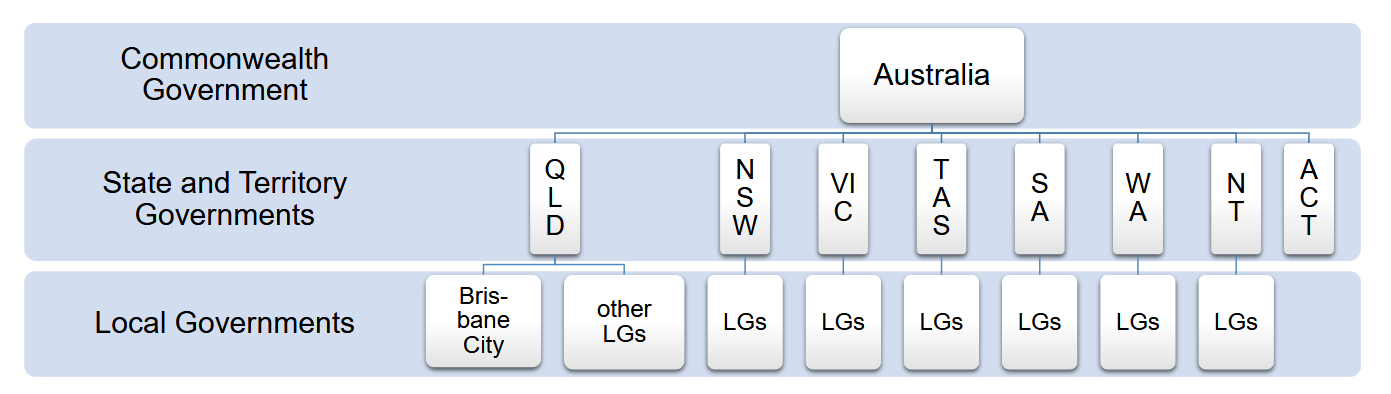
\includegraphics[width=0.8\textwidth]{images/figures/govstructure.png}
		\caption{Australian Governance Structure}
		\label{fig:your_label}
	\end{figure}

	\begin{figure}[htbp]
		\centering
		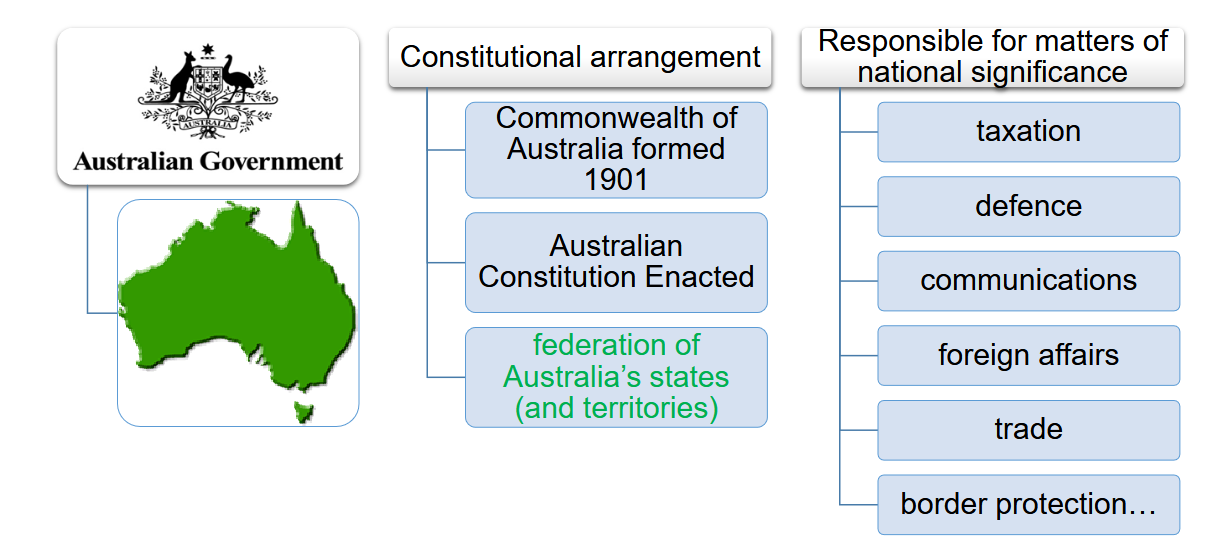
\includegraphics[width=0.47\textwidth]{images/figures/Comgov.png}
		\hfill
		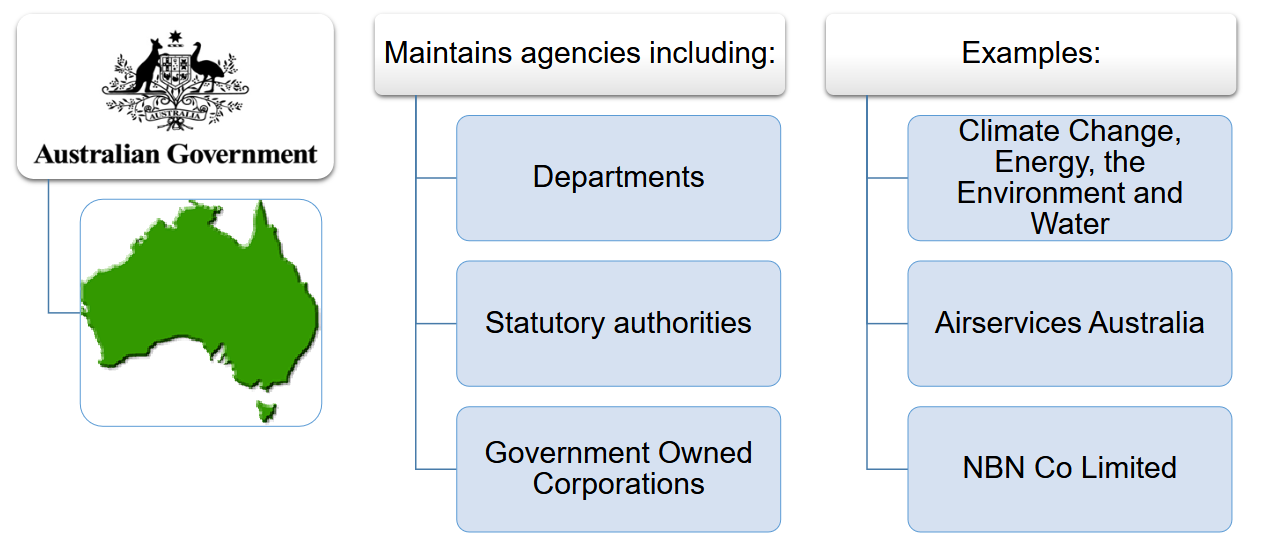
\includegraphics[width=0.47\textwidth]{images/figures/comgov2.png}
		\caption{Commonwealth Government}
		\label{fig:two_images}
	\end{figure}

	\begin{figure}[htbp]
		\centering
		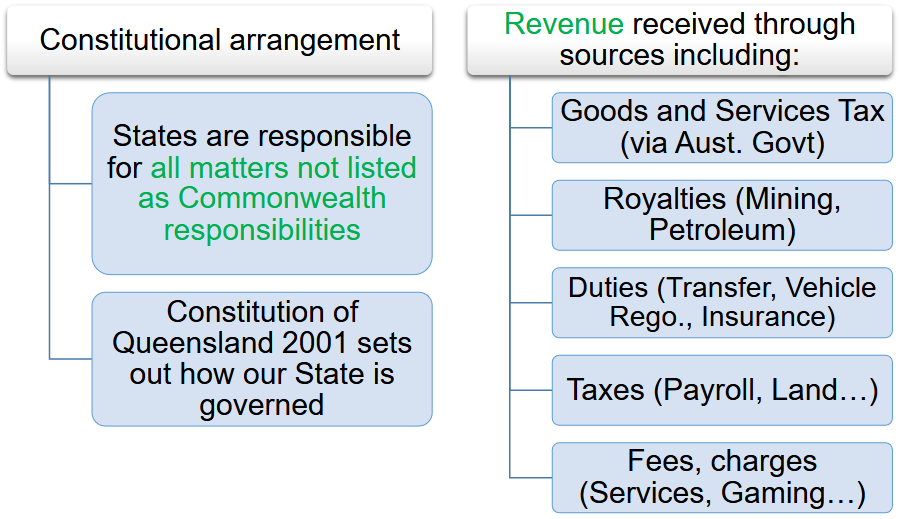
\includegraphics[width=0.47\textwidth]{images/figures/state1.png}
		\hfill
		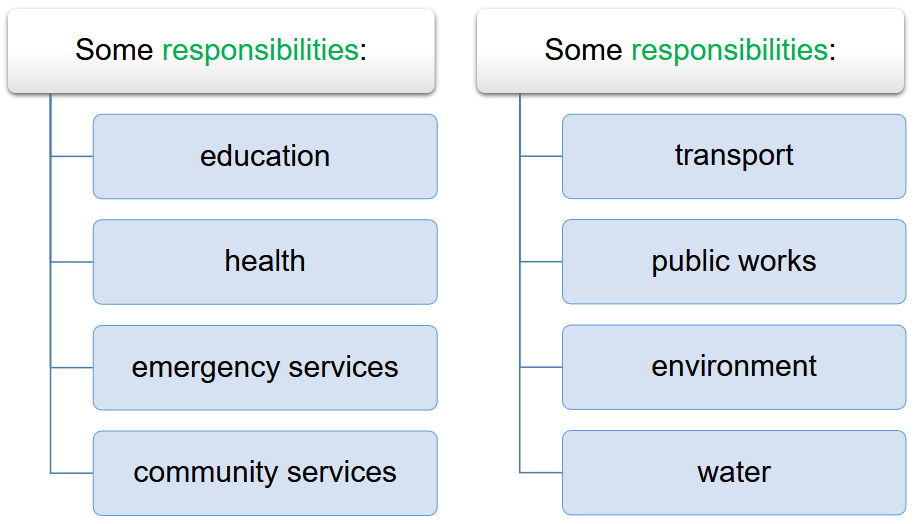
\includegraphics[width=0.47\textwidth]{images/figures/state2.png}
		\caption{State Government}
		\label{fig:two_images}
	\end{figure}

	\subsection{Local Government}
	\begin{itemize}
		\item Local Government is the lowest lay of government, but by no means the least important
		\item Many states maintain small local governments (suburbs etc)
		\item Queensland maintains larger LGs called city councils or regional councils. Larger LGs tend to be more economical. 
		\item Revenue is recieved through sources including council rates, fees, charges for services (rubbish collects etc) and grants from higher levels of government. 
		\item Some responsibilites include:
		\begin{itemize}
			\item Preparation and Stewardship of Planning Scheme
			\item Provision of ceratin infrastructure and services
			\item Regulation of certain activities
			\item Examples of this include land zoning, planning, streets, some roads, waste management, parks, building approcials, food health regulation and parking.
		\end{itemize}
	\end{itemize}

	\subsection{Brisbane City Vision}
	The vision of Brisbane is the outline of goals and desired outcomes for the development and state of the city in relation to communties view as and long term plans. THe brisbane vision is the long term plans and other strategies put in place to address planning for the future. 
	
	\subsubsection{Vision and Roles}
	\begin{itemize}
		\item Regulates certain activities
		\item Provides services
		\item Funds other organisations to deliver services
		\item Partners and alliances with other parties in community interests
		\item Facilities others to be involved in activites by bringing groups and other parties together
		\item Advocated by promoting community interests to other influencers and decision makers. 
	\end{itemize}

	\subsection{Professional Associations}
	The Australian Competition and Consumer Commission
	\begin{itemize}
		\item help educate members, maintaining high standards and ethical behaviour
		\item can develop their own codes of conduct or voluntary professional rules
		\item must comply with the Competition and Consumer Act 2010
	\end{itemize}

	\begin{figure}[htbp]
		\centering
		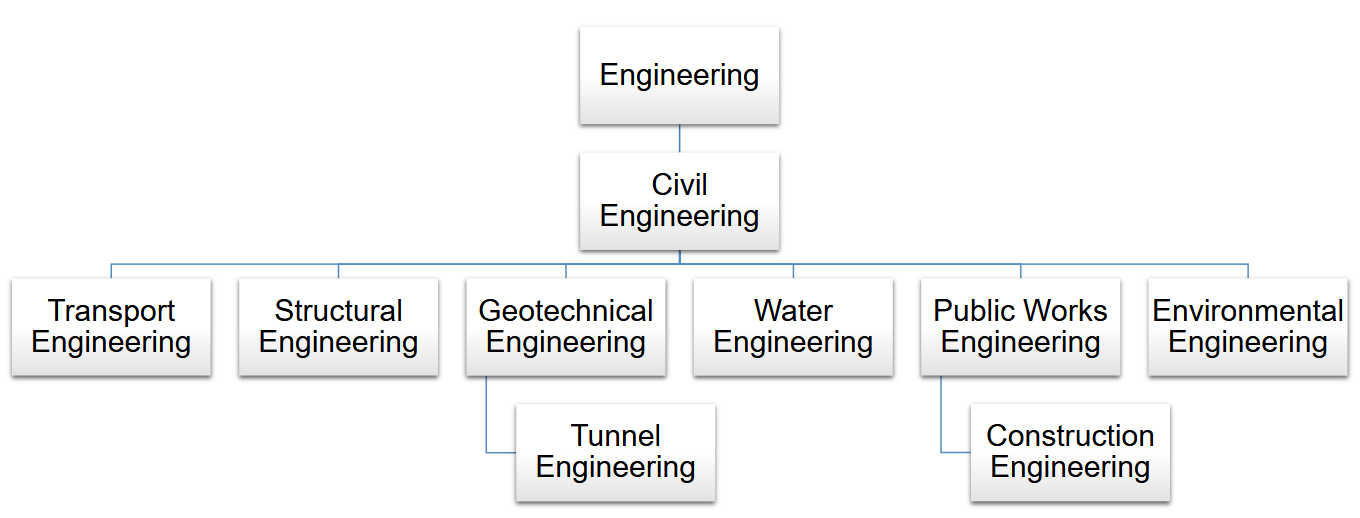
\includegraphics[width=0.8\textwidth]{images/figures/ENGDIS.png}
		\caption{Australian Civil Engineering and its Sub-disciplines}
		\label{fig:your_label}
	\end{figure}

	Why may civil engineers need professional associations?

	\begin{itemize}
		\item They provide for stable governance to ensure consistently high standards of engineering practice
		\item They promote the ongoing engagement of each individual engineer with whole Engineering Team
		\item They provide a well-informed voice on engineering issues important to wellbeing of wider community
		\item They foster Change when appropriate, and help Engineering Team to manage Change that comes to us
	\end{itemize}

	\newpage
	\subsection{Civil Engineering Sphere of Influence for an Urban Study Area}
	\begin{figure}[htbp]
		\centering
		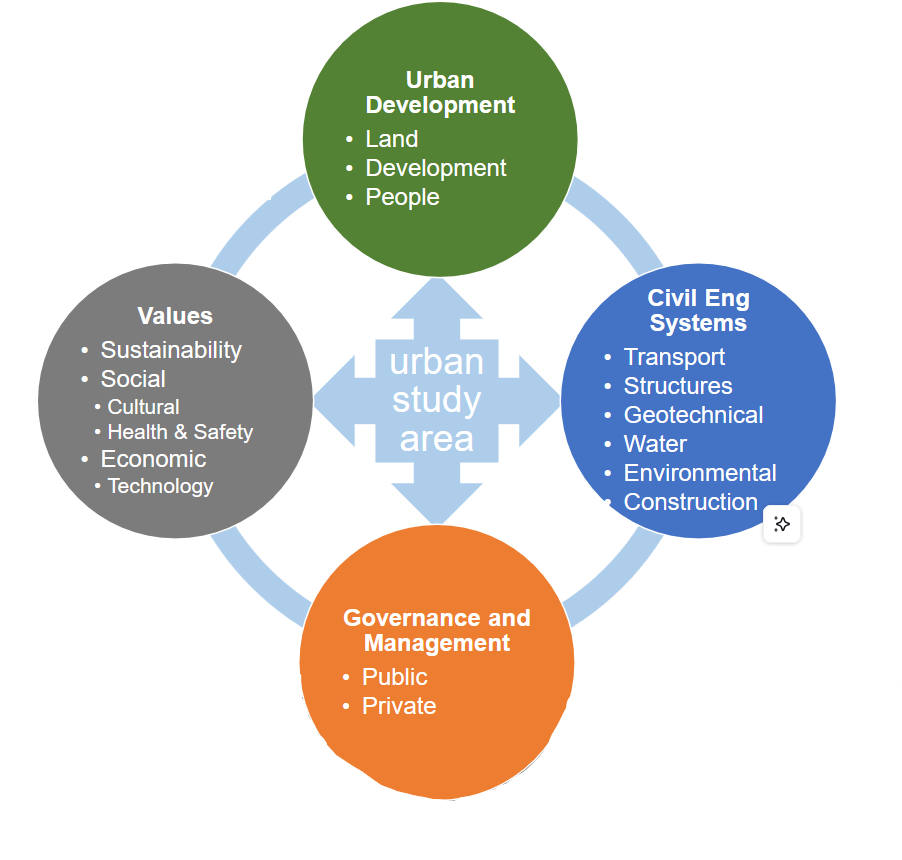
\includegraphics[width=0.8\textwidth]{images/figures/sphere.png}
		\caption{Sphere of Influence}
		\label{fig:your_label}
	\end{figure}

	\newpage
	\thm{Theorem Name}{Theorem Statement}
	\cor[cori]{Corollary Name}{Corollary Statement}
	\lem{Lemma Name}{Lemma Statement}
	\clm{Claim Name}{Claim Statement}
	\ex{Example Name}{Example explained}


	\opn{Open Question Name}{Question Statement}
%\qs{Question Name}{Question Statement}
\nt{Special Note}
\wc{Wrong Concept topic}{Explanation}
%\pf{Proof}{Proof}
	
\chapter{Second Chapter}
\section{Section 1}
\end{document}